\documentclass{article}
\usepackage[spanish]{babel}
\usepackage{graphicx} % Paquete necesario para imágenes

\begin{document}

\title{Variables y Límites en la Producción de Papa en Perú}
\author{Kenny Leonel Ccora-Quispe}
\date{\today}
\maketitle

\section{Introducción}
Según el \textbf{Ministerio de Agricultura (MINAGRI, 2020)} \cite{minagri2020}, Perú es el primer productor de papa en América Latina, con una producción anual de \textbf{5.3 millones de toneladas} y un rendimiento promedio de \textbf{16.1 toneladas por hectárea}.

% Aquí insertamos la imagen
\begin{center}
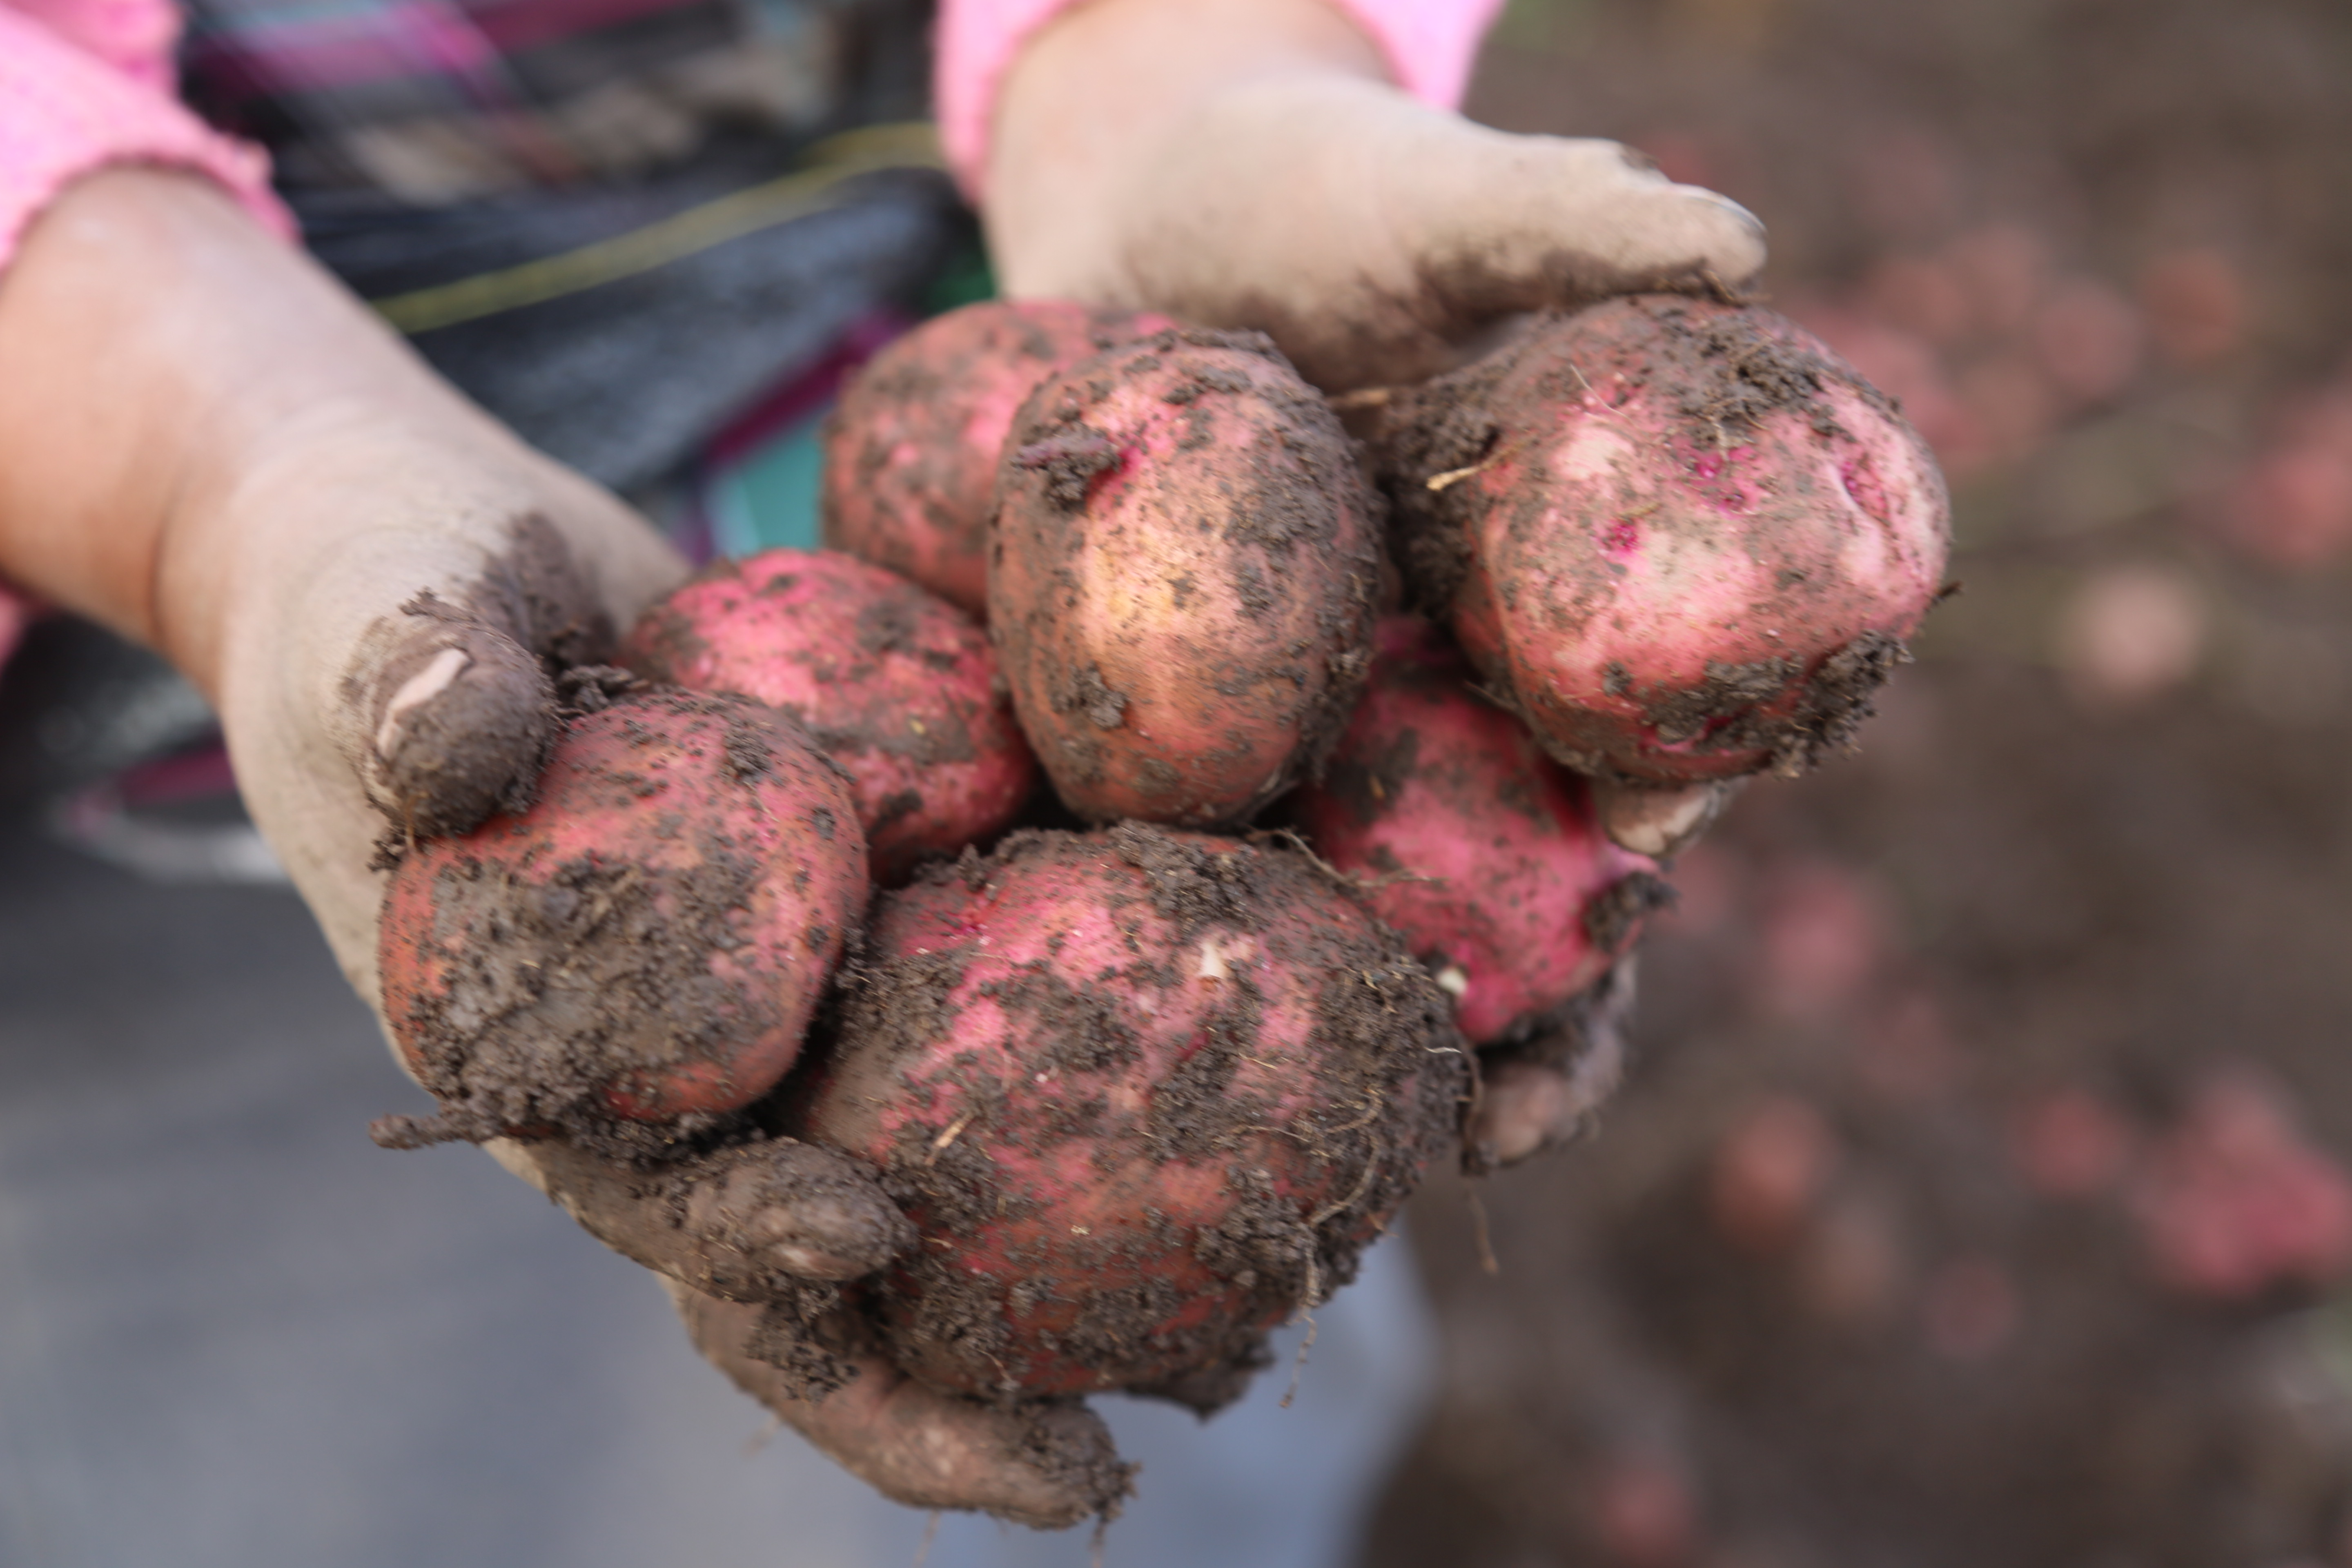
\includegraphics[width=0.8\textwidth]{la_papa.jpg} % Cambia el nombre de la imagen
\end{center}

\section{Variables}
\begin{itemize}
    \item \textbf{Producción Total (P)}: Toneladas de papa/año.
    \item \textbf{Área Cultivada (A)}: Hectáreas dedicadas al cultivo.
\end{itemize}

\section{Función}
El rendimiento promedio (R) se calcula como:
\[
R = \frac{P}{A} = \frac{5,300,000\ \text{ton}}{330,000\ \text{ha}} \approx 16.1\ \text{ton/ha}
\]

\section{Límites}
\begin{itemize}
    \item Área máxima por agricultor: \textbf{10 ha} (ejemplo para pequeñas familias, ajustable según región).
    \item Rendimiento mínimo: \textbf{10 ton/ha} (para ser rentable, según expertos)
    \item Límite: 5.3 millones de toneladas (dato MINAGRI 2019).
    \item Límite: 330,000 ha (total nacional reportado).
\end{itemize}

\begin{thebibliography}{9}
\bibitem{minagri2020} 
MINAGRI. (2020). ``Perú es primer productor de papa en América Latina''. \\
\emph{Oficina de Comunicaciones}. Disponible en: \\
\url{https://www.gob.pe/institucion/minagri/noticias/236419-peru-se-mantiene-como-primer-productor-de-papa-en-america-latina}
\end{thebibliography}

\end{document}